% Created by tikzDevice version 0.8.1 on 2015-03-24 11:04:29
% !TEX encoding = UTF-8 Unicode
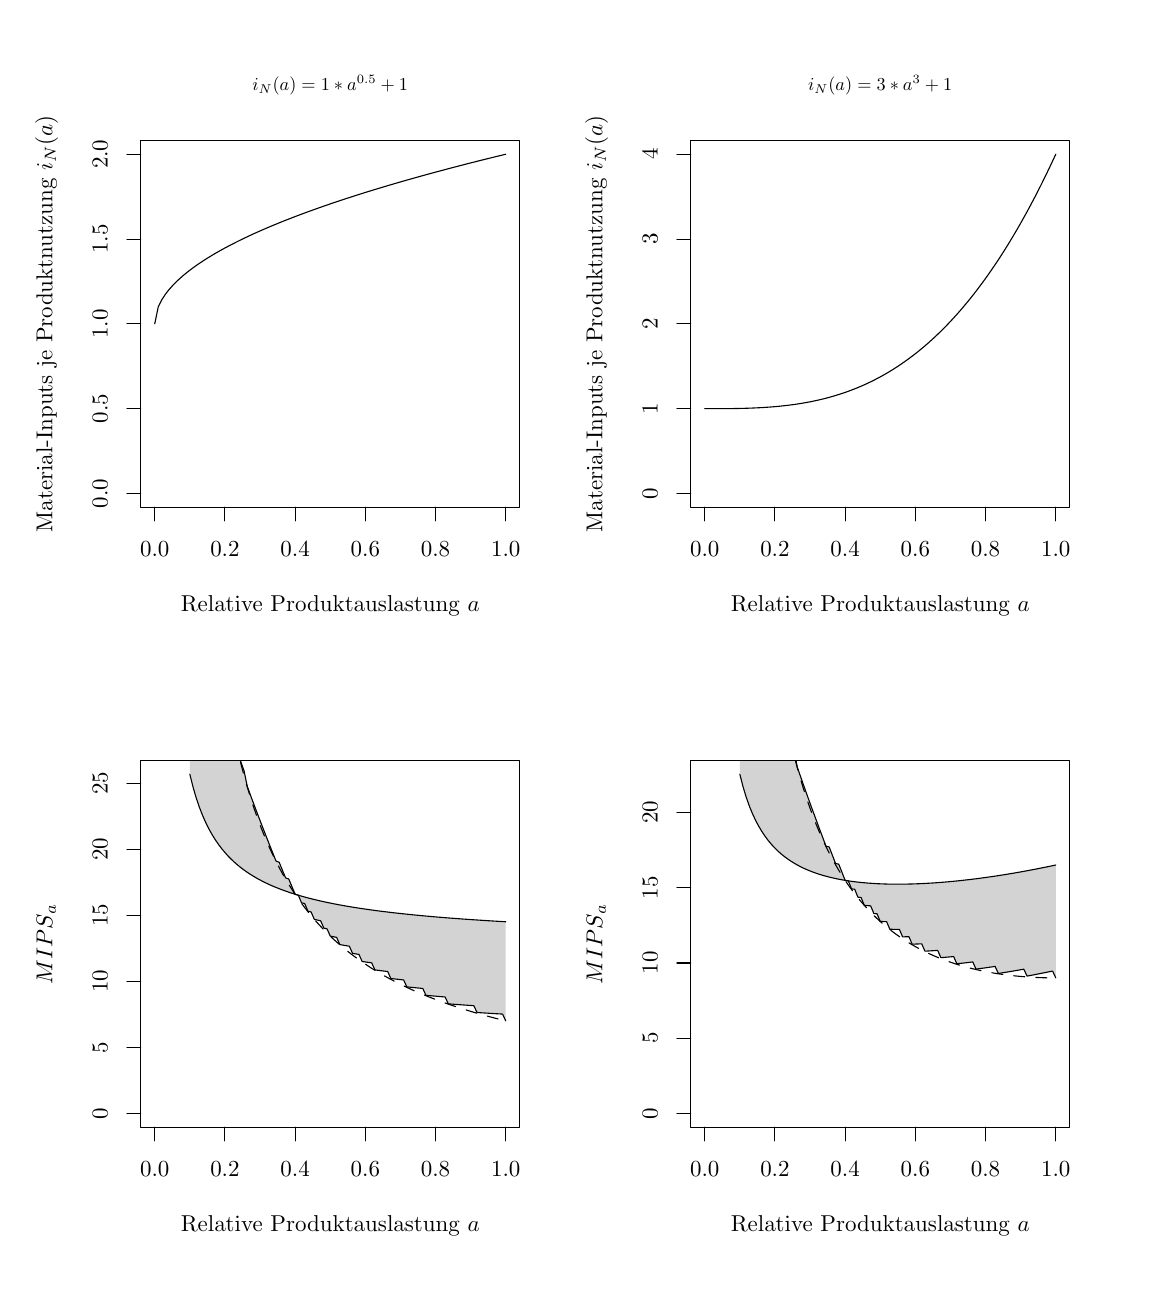
\begin{tikzpicture}[x=1pt,y=1pt]
\definecolor{fillColor}{RGB}{255,255,255}
\path[use as bounding box,fill=fillColor,fill opacity=0.00] (0,0) rectangle (397.48,448.07);
\begin{scope}
\path[clip] ( 40.84,274.83) rectangle (177.83,407.24);
\definecolor{drawColor}{RGB}{0,0,0}

\path[draw=drawColor,line width= 0.4pt,line join=round,line cap=round] ( 45.91,341.04) --
	( 47.19,347.20) --
	( 48.47,349.75) --
	( 49.75,351.71) --
	( 51.03,353.36) --
	( 52.32,354.81) --
	( 53.60,356.13) --
	( 54.88,357.34) --
	( 56.16,358.46) --
	( 57.44,359.52) --
	( 58.72,360.52) --
	( 60.00,361.47) --
	( 61.28,362.38) --
	( 62.57,363.25) --
	( 63.85,364.09) --
	( 65.13,364.90) --
	( 66.41,365.68) --
	( 67.69,366.44) --
	( 68.97,367.17) --
	( 70.25,367.89) --
	( 71.53,368.59) --
	( 72.82,369.27) --
	( 74.10,369.93) --
	( 75.38,370.58) --
	( 76.66,371.22) --
	( 77.94,371.84) --
	( 79.22,372.45) --
	( 80.50,373.05) --
	( 81.78,373.64) --
	( 83.07,374.21) --
	( 84.35,374.78) --
	( 85.63,375.34) --
	( 86.91,375.89) --
	( 88.19,376.43) --
	( 89.47,376.96) --
	( 90.75,377.48) --
	( 92.03,378.00) --
	( 93.32,378.51) --
	( 94.60,379.01) --
	( 95.88,379.51) --
	( 97.16,380.00) --
	( 98.44,380.48) --
	( 99.72,380.96) --
	(101.00,381.43) --
	(102.28,381.90) --
	(103.57,382.36) --
	(104.85,382.82) --
	(106.13,383.27) --
	(107.41,383.72) --
	(108.69,384.16) --
	(109.97,384.60) --
	(111.25,385.03) --
	(112.53,385.46) --
	(113.82,385.89) --
	(115.10,386.31) --
	(116.38,386.72) --
	(117.66,387.14) --
	(118.94,387.55) --
	(120.22,387.95) --
	(121.50,388.36) --
	(122.78,388.76) --
	(124.07,389.15) --
	(125.35,389.55) --
	(126.63,389.93) --
	(127.91,390.32) --
	(129.19,390.70) --
	(130.47,391.09) --
	(131.75,391.46) --
	(133.03,391.84) --
	(134.32,392.21) --
	(135.60,392.58) --
	(136.88,392.95) --
	(138.16,393.31) --
	(139.44,393.67) --
	(140.72,394.03) --
	(142.00,394.39) --
	(143.28,394.74) --
	(144.57,395.10) --
	(145.85,395.45) --
	(147.13,395.79) --
	(148.41,396.14) --
	(149.69,396.48) --
	(150.97,396.82) --
	(152.25,397.16) --
	(153.53,397.50) --
	(154.82,397.83) --
	(156.10,398.17) --
	(157.38,398.50) --
	(158.66,398.83) --
	(159.94,399.16) --
	(161.22,399.48) --
	(162.50,399.81) --
	(163.78,400.13) --
	(165.07,400.45) --
	(166.35,400.77) --
	(167.63,401.08) --
	(168.91,401.40) --
	(170.19,401.71) --
	(171.47,402.02) --
	(172.75,402.33);
\end{scope}
\begin{scope}
\path[clip] (  0.00,  0.00) rectangle (397.48,448.07);
\definecolor{drawColor}{RGB}{0,0,0}

\path[draw=drawColor,line width= 0.4pt,line join=round,line cap=round] ( 45.91,274.83) -- (172.75,274.83);

\path[draw=drawColor,line width= 0.4pt,line join=round,line cap=round] ( 45.91,274.83) -- ( 45.91,269.85);

\path[draw=drawColor,line width= 0.4pt,line join=round,line cap=round] ( 71.28,274.83) -- ( 71.28,269.85);

\path[draw=drawColor,line width= 0.4pt,line join=round,line cap=round] ( 96.65,274.83) -- ( 96.65,269.85);

\path[draw=drawColor,line width= 0.4pt,line join=round,line cap=round] (122.02,274.83) -- (122.02,269.85);

\path[draw=drawColor,line width= 0.4pt,line join=round,line cap=round] (147.38,274.83) -- (147.38,269.85);

\path[draw=drawColor,line width= 0.4pt,line join=round,line cap=round] (172.75,274.83) -- (172.75,269.85);

\node[text=drawColor,anchor=base,inner sep=0pt, outer sep=0pt, scale=  0.83] at ( 45.91,256.90) {0.0};

\node[text=drawColor,anchor=base,inner sep=0pt, outer sep=0pt, scale=  0.83] at ( 71.28,256.90) {0.2};

\node[text=drawColor,anchor=base,inner sep=0pt, outer sep=0pt, scale=  0.83] at ( 96.65,256.90) {0.4};

\node[text=drawColor,anchor=base,inner sep=0pt, outer sep=0pt, scale=  0.83] at (122.02,256.90) {0.6};

\node[text=drawColor,anchor=base,inner sep=0pt, outer sep=0pt, scale=  0.83] at (147.38,256.90) {0.8};

\node[text=drawColor,anchor=base,inner sep=0pt, outer sep=0pt, scale=  0.83] at (172.75,256.90) {1.0};

\path[draw=drawColor,line width= 0.4pt,line join=round,line cap=round] ( 40.84,279.74) -- ( 40.84,402.33);

\path[draw=drawColor,line width= 0.4pt,line join=round,line cap=round] ( 40.84,279.74) -- ( 35.86,279.74);

\path[draw=drawColor,line width= 0.4pt,line join=round,line cap=round] ( 40.84,310.39) -- ( 35.86,310.39);

\path[draw=drawColor,line width= 0.4pt,line join=round,line cap=round] ( 40.84,341.04) -- ( 35.86,341.04);

\path[draw=drawColor,line width= 0.4pt,line join=round,line cap=round] ( 40.84,371.68) -- ( 35.86,371.68);

\path[draw=drawColor,line width= 0.4pt,line join=round,line cap=round] ( 40.84,402.33) -- ( 35.86,402.33);

\node[text=drawColor,rotate= 90.00,anchor=base,inner sep=0pt, outer sep=0pt, scale=  0.83] at ( 28.88,279.74) {0.0};

\node[text=drawColor,rotate= 90.00,anchor=base,inner sep=0pt, outer sep=0pt, scale=  0.83] at ( 28.88,310.39) {0.5};

\node[text=drawColor,rotate= 90.00,anchor=base,inner sep=0pt, outer sep=0pt, scale=  0.83] at ( 28.88,341.04) {1.0};

\node[text=drawColor,rotate= 90.00,anchor=base,inner sep=0pt, outer sep=0pt, scale=  0.83] at ( 28.88,371.68) {1.5};

\node[text=drawColor,rotate= 90.00,anchor=base,inner sep=0pt, outer sep=0pt, scale=  0.83] at ( 28.88,402.33) {2.0};

\path[draw=drawColor,line width= 0.4pt,line join=round,line cap=round] ( 40.84,274.83) --
	(177.83,274.83) --
	(177.83,407.24) --
	( 40.84,407.24) --
	( 40.84,274.83);
\end{scope}
\begin{scope}
\path[clip] (  0.00,224.04) rectangle (198.74,448.07);
\definecolor{drawColor}{RGB}{0,0,0}

\node[text=drawColor,anchor=base,inner sep=0pt, outer sep=0pt, scale=  0.83] at (109.33,236.99) {Relative Produktauslastung $a$};

\node[text=drawColor,rotate= 90.00,anchor=base,inner sep=0pt, outer sep=0pt, scale=  0.83] at (  8.96,341.04) {Material-Inputs je Produktnutzung $i_N(a)$};

\node[text=drawColor,anchor=base,inner sep=0pt, outer sep=0pt, scale=  0.66] at (109.33,425.36) {\bfseries $i_N(a) = 1* a^{0.5}+1$};
\end{scope}
\begin{scope}
\path[clip] ( 40.84, 50.80) rectangle (177.83,183.20);
\definecolor{fillColor}{RGB}{211,211,211}

\path[fill=fillColor] ( 58.59,357.38) --
	( 59.75,333.65) --
	( 60.90,313.00) --
	( 62.05,295.29) --
	( 63.21,280.39) --
	( 64.36,265.85) --
	( 65.51,254.00) --
	( 66.67,244.78) --
	( 67.82,233.37) --
	( 68.97,224.54) --
	( 70.13,218.24) --
	( 71.28,209.69) --
	( 72.43,203.64) --
	( 73.58,197.69) --
	( 74.74,194.22) --
	( 75.89,188.45) --
	( 77.04,182.74) --
	( 78.20,179.48) --
	( 79.35,173.90) --
	( 80.50,170.75) --
	( 81.66,167.65) --
	( 82.81,164.59) --
	( 83.96,161.57) --
	( 85.12,158.58) --
	( 86.27,155.63) --
	( 87.42,152.71) --
	( 88.58,149.81) --
	( 89.73,146.94) --
	( 90.88,146.48) --
	( 92.03,143.66) --
	( 93.19,140.85) --
	( 94.34,140.45) --
	( 95.49,137.68) --
	( 96.65,134.93) --
	( 97.80,134.58) --
	( 98.95,134.25) --
	(100.11,133.92) --
	(101.26,133.61) --
	(102.41,133.32) --
	(103.57,133.03) --
	(104.72,132.75) --
	(105.87,132.49) --
	(107.03,132.23) --
	(108.18,131.98) --
	(109.33,131.75) --
	(110.48,131.51) --
	(111.64,131.29) --
	(112.79,131.07) --
	(113.94,130.87) --
	(115.10,130.66) --
	(116.25,130.47) --
	(117.40,130.27) --
	(118.56,130.09) --
	(119.71,129.91) --
	(120.86,129.73) --
	(122.02,129.57) --
	(123.17,129.40) --
	(124.32,129.24) --
	(125.47,129.08) --
	(126.63,128.93) --
	(127.78,128.78) --
	(128.93,128.64) --
	(130.09,128.50) --
	(131.24,128.36) --
	(132.39,128.23) --
	(133.55,128.10) --
	(134.70,127.97) --
	(135.85,127.85) --
	(137.01,127.73) --
	(138.16,127.61) --
	(139.31,127.49) --
	(140.47,127.38) --
	(141.62,127.27) --
	(142.77,127.16) --
	(143.92,127.05) --
	(145.08,126.95) --
	(146.23,126.85) --
	(147.38,126.75) --
	(148.54,126.65) --
	(149.69,126.56) --
	(150.84,126.46) --
	(152.00,126.37) --
	(153.15,126.28) --
	(154.30,126.20) --
	(155.46,126.11) --
	(156.61,126.02) --
	(157.76,125.94) --
	(158.92,125.86) --
	(160.07,125.78) --
	(161.22,125.70) --
	(162.37,125.63) --
	(163.53,125.55) --
	(164.68,125.48) --
	(165.83,125.40) --
	(166.99,125.33) --
	(168.14,125.26) --
	(169.29,125.19) --
	(170.45,125.12) --
	(171.60,125.06) --
	(172.75,124.99) --
	(172.75, 89.18) --
	(171.60, 91.63) --
	(170.45, 91.70) --
	(169.29, 91.76) --
	(168.14, 91.83) --
	(166.99, 91.90) --
	(165.83, 91.98) --
	(164.68, 92.05) --
	(163.53, 92.12) --
	(162.37, 92.20) --
	(161.22, 94.66) --
	(160.07, 94.74) --
	(158.92, 94.82) --
	(157.76, 94.90) --
	(156.61, 94.98) --
	(155.46, 95.07) --
	(154.30, 95.15) --
	(153.15, 95.24) --
	(152.00, 95.33) --
	(150.84, 97.81) --
	(149.69, 97.90) --
	(148.54, 98.00) --
	(147.38, 98.10) --
	(146.23, 98.20) --
	(145.08, 98.30) --
	(143.92, 98.40) --
	(142.77,100.89) --
	(141.62,101.00) --
	(140.47,101.11) --
	(139.31,101.23) --
	(138.16,101.34) --
	(137.01,101.46) --
	(135.85,103.97) --
	(134.70,104.09) --
	(133.55,104.22) --
	(132.39,104.35) --
	(131.24,104.48) --
	(130.09,107.01) --
	(128.93,107.15) --
	(127.78,107.29) --
	(126.63,107.44) --
	(125.47,107.59) --
	(124.32,110.14) --
	(123.17,110.30) --
	(122.02,110.46) --
	(120.86,110.63) --
	(119.71,113.20) --
	(118.56,113.38) --
	(117.40,113.56) --
	(116.25,116.14) --
	(115.10,116.34) --
	(113.94,116.54) --
	(112.79,116.75) --
	(111.64,119.35) --
	(110.48,119.58) --
	(109.33,119.81) --
	(108.18,122.43) --
	(107.03,122.68) --
	(105.87,125.33) --
	(104.72,125.59) --
	(103.57,125.87) --
	(102.41,128.54) --
	(101.26,128.84) --
	(100.11,131.54) --
	( 98.95,131.86) --
	( 97.80,134.58) --
	( 96.65,134.93) --
	( 95.49,135.30) --
	( 94.34,135.68) --
	( 93.19,136.08) --
	( 92.03,136.49) --
	( 90.88,136.93) --
	( 89.73,137.39) --
	( 88.58,137.87) --
	( 87.42,138.38) --
	( 86.27,138.92) --
	( 85.12,139.48) --
	( 83.96,140.08) --
	( 82.81,140.71) --
	( 81.66,141.38) --
	( 80.50,142.10) --
	( 79.35,142.86) --
	( 78.20,143.67) --
	( 77.04,144.54) --
	( 75.89,145.47) --
	( 74.74,146.47) --
	( 73.58,147.55) --
	( 72.43,148.72) --
	( 71.28,150.00) --
	( 70.13,151.38) --
	( 68.97,152.91) --
	( 67.82,154.58) --
	( 66.67,156.43) --
	( 65.51,158.49) --
	( 64.36,160.79) --
	( 63.21,163.39) --
	( 62.05,166.35) --
	( 60.90,169.74) --
	( 59.75,173.67) --
	( 58.59,178.30) --
	cycle;
\definecolor{drawColor}{RGB}{0,0,0}

\path[draw=drawColor,line width= 0.4pt,line join=round,line cap=round] ( 58.59,178.30) --
	( 59.75,173.67) --
	( 60.90,169.74) --
	( 62.05,166.35) --
	( 63.21,163.39) --
	( 64.36,160.79) --
	( 65.51,158.49) --
	( 66.67,156.43) --
	( 67.82,154.58) --
	( 68.97,152.91) --
	( 70.13,151.38) --
	( 71.28,150.00) --
	( 72.43,148.72) --
	( 73.58,147.55) --
	( 74.74,146.47) --
	( 75.89,145.47) --
	( 77.04,144.54) --
	( 78.20,143.67) --
	( 79.35,142.86) --
	( 80.50,142.10) --
	( 81.66,141.38) --
	( 82.81,140.71) --
	( 83.96,140.08) --
	( 85.12,139.48) --
	( 86.27,138.92) --
	( 87.42,138.38) --
	( 88.58,137.87) --
	( 89.73,137.39) --
	( 90.88,136.93) --
	( 92.03,136.49) --
	( 93.19,136.08) --
	( 94.34,135.68) --
	( 95.49,135.30) --
	( 96.65,134.93) --
	( 97.80,134.58) --
	( 98.95,134.25) --
	(100.11,133.92) --
	(101.26,133.61) --
	(102.41,133.32) --
	(103.57,133.03) --
	(104.72,132.75) --
	(105.87,132.49) --
	(107.03,132.23) --
	(108.18,131.98) --
	(109.33,131.75) --
	(110.48,131.51) --
	(111.64,131.29) --
	(112.79,131.07) --
	(113.94,130.87) --
	(115.10,130.66) --
	(116.25,130.47) --
	(117.40,130.27) --
	(118.56,130.09) --
	(119.71,129.91) --
	(120.86,129.73) --
	(122.02,129.57) --
	(123.17,129.40) --
	(124.32,129.24) --
	(125.47,129.08) --
	(126.63,128.93) --
	(127.78,128.78) --
	(128.93,128.64) --
	(130.09,128.50) --
	(131.24,128.36) --
	(132.39,128.23) --
	(133.55,128.10) --
	(134.70,127.97) --
	(135.85,127.85) --
	(137.01,127.73) --
	(138.16,127.61) --
	(139.31,127.49) --
	(140.47,127.38) --
	(141.62,127.27) --
	(142.77,127.16) --
	(143.92,127.05) --
	(145.08,126.95) --
	(146.23,126.85) --
	(147.38,126.75) --
	(148.54,126.65) --
	(149.69,126.56) --
	(150.84,126.46) --
	(152.00,126.37) --
	(153.15,126.28) --
	(154.30,126.20) --
	(155.46,126.11) --
	(156.61,126.02) --
	(157.76,125.94) --
	(158.92,125.86) --
	(160.07,125.78) --
	(161.22,125.70) --
	(162.37,125.63) --
	(163.53,125.55) --
	(164.68,125.48) --
	(165.83,125.40) --
	(166.99,125.33) --
	(168.14,125.26) --
	(169.29,125.19) --
	(170.45,125.12) --
	(171.60,125.06) --
	(172.75,124.99);
\end{scope}
\begin{scope}
\path[clip] (  0.00,  0.00) rectangle (397.48,448.07);
\definecolor{drawColor}{RGB}{0,0,0}

\path[draw=drawColor,line width= 0.4pt,line join=round,line cap=round] ( 45.91, 50.80) -- (172.75, 50.80);

\path[draw=drawColor,line width= 0.4pt,line join=round,line cap=round] ( 45.91, 50.80) -- ( 45.91, 45.82);

\path[draw=drawColor,line width= 0.4pt,line join=round,line cap=round] ( 71.28, 50.80) -- ( 71.28, 45.82);

\path[draw=drawColor,line width= 0.4pt,line join=round,line cap=round] ( 96.65, 50.80) -- ( 96.65, 45.82);

\path[draw=drawColor,line width= 0.4pt,line join=round,line cap=round] (122.02, 50.80) -- (122.02, 45.82);

\path[draw=drawColor,line width= 0.4pt,line join=round,line cap=round] (147.38, 50.80) -- (147.38, 45.82);

\path[draw=drawColor,line width= 0.4pt,line join=round,line cap=round] (172.75, 50.80) -- (172.75, 45.82);

\node[text=drawColor,anchor=base,inner sep=0pt, outer sep=0pt, scale=  0.83] at ( 45.91, 32.87) {0.0};

\node[text=drawColor,anchor=base,inner sep=0pt, outer sep=0pt, scale=  0.83] at ( 71.28, 32.87) {0.2};

\node[text=drawColor,anchor=base,inner sep=0pt, outer sep=0pt, scale=  0.83] at ( 96.65, 32.87) {0.4};

\node[text=drawColor,anchor=base,inner sep=0pt, outer sep=0pt, scale=  0.83] at (122.02, 32.87) {0.6};

\node[text=drawColor,anchor=base,inner sep=0pt, outer sep=0pt, scale=  0.83] at (147.38, 32.87) {0.8};

\node[text=drawColor,anchor=base,inner sep=0pt, outer sep=0pt, scale=  0.83] at (172.75, 32.87) {1.0};

\path[draw=drawColor,line width= 0.4pt,line join=round,line cap=round] ( 40.84, 55.70) -- ( 40.84,175.09);

\path[draw=drawColor,line width= 0.4pt,line join=round,line cap=round] ( 40.84, 55.70) -- ( 35.86, 55.70);

\path[draw=drawColor,line width= 0.4pt,line join=round,line cap=round] ( 40.84, 79.58) -- ( 35.86, 79.58);

\path[draw=drawColor,line width= 0.4pt,line join=round,line cap=round] ( 40.84,103.45) -- ( 35.86,103.45);

\path[draw=drawColor,line width= 0.4pt,line join=round,line cap=round] ( 40.84,127.33) -- ( 35.86,127.33);

\path[draw=drawColor,line width= 0.4pt,line join=round,line cap=round] ( 40.84,151.21) -- ( 35.86,151.21);

\path[draw=drawColor,line width= 0.4pt,line join=round,line cap=round] ( 40.84,175.09) -- ( 35.86,175.09);

\node[text=drawColor,rotate= 90.00,anchor=base,inner sep=0pt, outer sep=0pt, scale=  0.83] at ( 28.88, 55.70) {0};

\node[text=drawColor,rotate= 90.00,anchor=base,inner sep=0pt, outer sep=0pt, scale=  0.83] at ( 28.88, 79.58) {5};

\node[text=drawColor,rotate= 90.00,anchor=base,inner sep=0pt, outer sep=0pt, scale=  0.83] at ( 28.88,103.45) {10};

\node[text=drawColor,rotate= 90.00,anchor=base,inner sep=0pt, outer sep=0pt, scale=  0.83] at ( 28.88,127.33) {15};

\node[text=drawColor,rotate= 90.00,anchor=base,inner sep=0pt, outer sep=0pt, scale=  0.83] at ( 28.88,151.21) {20};

\node[text=drawColor,rotate= 90.00,anchor=base,inner sep=0pt, outer sep=0pt, scale=  0.83] at ( 28.88,175.09) {25};

\path[draw=drawColor,line width= 0.4pt,line join=round,line cap=round] ( 40.84, 50.80) --
	(177.83, 50.80) --
	(177.83,183.20) --
	( 40.84,183.20) --
	( 40.84, 50.80);
\end{scope}
\begin{scope}
\path[clip] (  0.00,  0.00) rectangle (198.74,224.04);
\definecolor{drawColor}{RGB}{0,0,0}

\node[text=drawColor,anchor=base,inner sep=0pt, outer sep=0pt, scale=  0.83] at (109.33, 12.95) {Relative Produktauslastung $a$};

\node[text=drawColor,rotate= 90.00,anchor=base,inner sep=0pt, outer sep=0pt, scale=  0.83] at (  8.96,117.00) {$\text{MIPS}_a$};
\end{scope}
\begin{scope}
\path[clip] ( 40.84, 50.80) rectangle (177.83,183.20);
\definecolor{drawColor}{RGB}{0,0,0}

\path[draw=drawColor,line width= 0.4pt,dash pattern=on 4pt off 4pt ,line join=round,line cap=round] ( 58.59,357.38) --
	( 59.75,332.86) --
	( 60.90,312.09) --
	( 62.05,294.26) --
	( 63.21,278.80) --
	( 64.36,265.26) --
	( 65.51,253.30) --
	( 66.67,242.65) --
	( 67.82,233.12) --
	( 68.97,224.54) --
	( 70.13,216.76) --
	( 71.28,209.69) --
	( 72.43,203.23) --
	( 73.58,197.30) --
	( 74.74,191.84) --
	( 75.89,186.79) --
	( 77.04,182.12) --
	( 78.20,177.78) --
	( 79.35,173.73) --
	( 80.50,169.95) --
	( 81.66,166.41) --
	( 82.81,163.10) --
	( 83.96,159.98) --
	( 85.12,157.04) --
	( 86.27,154.27) --
	( 87.42,151.65) --
	( 88.58,149.17) --
	( 89.73,146.81) --
	( 90.88,144.58) --
	( 92.03,142.46) --
	( 93.19,140.44) --
	( 94.34,138.52) --
	( 95.49,136.68) --
	( 96.65,134.93) --
	( 97.80,133.25) --
	( 98.95,131.65) --
	(100.11,130.11) --
	(101.26,128.64) --
	(102.41,127.23) --
	(103.57,125.87) --
	(104.72,124.56) --
	(105.87,123.31) --
	(107.03,122.10) --
	(108.18,120.93) --
	(109.33,119.81) --
	(110.48,118.72) --
	(111.64,117.68) --
	(112.79,116.67) --
	(113.94,115.69) --
	(115.10,114.74) --
	(116.25,113.83) --
	(117.40,112.94) --
	(118.56,112.09) --
	(119.71,111.26) --
	(120.86,110.45) --
	(122.02,109.67) --
	(123.17,108.91) --
	(124.32,108.17) --
	(125.47,107.46) --
	(126.63,106.76) --
	(127.78,106.08) --
	(128.93,105.43) --
	(130.09,104.79) --
	(131.24,104.16) --
	(132.39,103.56) --
	(133.55,102.96) --
	(134.70,102.39) --
	(135.85,101.83) --
	(137.01,101.28) --
	(138.16,100.75) --
	(139.31,100.22) --
	(140.47, 99.72) --
	(141.62, 99.22) --
	(142.77, 98.73) --
	(143.92, 98.26) --
	(145.08, 97.80) --
	(146.23, 97.35) --
	(147.38, 96.90) --
	(148.54, 96.47) --
	(149.69, 96.05) --
	(150.84, 95.63) --
	(152.00, 95.23) --
	(153.15, 94.83) --
	(154.30, 94.44) --
	(155.46, 94.06) --
	(156.61, 93.69) --
	(157.76, 93.33) --
	(158.92, 92.97) --
	(160.07, 92.62) --
	(161.22, 92.27) --
	(162.37, 91.94) --
	(163.53, 91.61) --
	(164.68, 91.28) --
	(165.83, 90.96) --
	(166.99, 90.65) --
	(168.14, 90.35) --
	(169.29, 90.05) --
	(170.45, 89.75) --
	(171.60, 89.46) --
	(172.75, 89.18);

\path[draw=drawColor,line width= 0.4pt,line join=round,line cap=round] ( 58.59,357.38) --
	( 59.75,333.65) --
	( 60.90,313.00) --
	( 62.05,295.29) --
	( 63.21,280.39) --
	( 64.36,265.85) --
	( 65.51,254.00) --
	( 66.67,244.78) --
	( 67.82,233.37) --
	( 68.97,224.54) --
	( 70.13,218.24) --
	( 71.28,209.69) --
	( 72.43,203.64) --
	( 73.58,197.69) --
	( 74.74,194.22) --
	( 75.89,188.45) --
	( 77.04,182.74) --
	( 78.20,179.48) --
	( 79.35,173.90) --
	( 80.50,170.75) --
	( 81.66,167.65) --
	( 82.81,164.59) --
	( 83.96,161.57) --
	( 85.12,158.58) --
	( 86.27,155.63) --
	( 87.42,152.71) --
	( 88.58,149.81) --
	( 89.73,146.94) --
	( 90.88,146.48) --
	( 92.03,143.66) --
	( 93.19,140.85) --
	( 94.34,140.45) --
	( 95.49,137.68) --
	( 96.65,134.93) --
	( 97.80,134.58) --
	( 98.95,131.86) --
	(100.11,131.54) --
	(101.26,128.84) --
	(102.41,128.54) --
	(103.57,125.87) --
	(104.72,125.59) --
	(105.87,125.33) --
	(107.03,122.68) --
	(108.18,122.43) --
	(109.33,119.81) --
	(110.48,119.58) --
	(111.64,119.35) --
	(112.79,116.75) --
	(113.94,116.54) --
	(115.10,116.34) --
	(116.25,116.14) --
	(117.40,113.56) --
	(118.56,113.38) --
	(119.71,113.20) --
	(120.86,110.63) --
	(122.02,110.46) --
	(123.17,110.30) --
	(124.32,110.14) --
	(125.47,107.59) --
	(126.63,107.44) --
	(127.78,107.29) --
	(128.93,107.15) --
	(130.09,107.01) --
	(131.24,104.48) --
	(132.39,104.35) --
	(133.55,104.22) --
	(134.70,104.09) --
	(135.85,103.97) --
	(137.01,101.46) --
	(138.16,101.34) --
	(139.31,101.23) --
	(140.47,101.11) --
	(141.62,101.00) --
	(142.77,100.89) --
	(143.92, 98.40) --
	(145.08, 98.30) --
	(146.23, 98.20) --
	(147.38, 98.10) --
	(148.54, 98.00) --
	(149.69, 97.90) --
	(150.84, 97.81) --
	(152.00, 95.33) --
	(153.15, 95.24) --
	(154.30, 95.15) --
	(155.46, 95.07) --
	(156.61, 94.98) --
	(157.76, 94.90) --
	(158.92, 94.82) --
	(160.07, 94.74) --
	(161.22, 94.66) --
	(162.37, 92.20) --
	(163.53, 92.12) --
	(164.68, 92.05) --
	(165.83, 91.98) --
	(166.99, 91.90) --
	(168.14, 91.83) --
	(169.29, 91.76) --
	(170.45, 91.70) --
	(171.60, 91.63) --
	(172.75, 89.18);
\end{scope}
\begin{scope}
\path[clip] (239.58,274.83) rectangle (376.57,407.24);
\definecolor{drawColor}{RGB}{0,0,0}

\path[draw=drawColor,line width= 0.4pt,line join=round,line cap=round] (244.65,310.39) --
	(245.93,310.39) --
	(247.21,310.39) --
	(248.50,310.39) --
	(249.78,310.39) --
	(251.06,310.40) --
	(252.34,310.41) --
	(253.62,310.42) --
	(254.90,310.43) --
	(256.18,310.46) --
	(257.46,310.48) --
	(258.75,310.51) --
	(260.03,310.55) --
	(261.31,310.59) --
	(262.59,310.65) --
	(263.87,310.71) --
	(265.15,310.77) --
	(266.43,310.85) --
	(267.71,310.94) --
	(269.00,311.04) --
	(270.28,311.14) --
	(271.56,311.26) --
	(272.84,311.40) --
	(274.12,311.54) --
	(275.40,311.70) --
	(276.68,311.87) --
	(277.96,312.05) --
	(279.25,312.25) --
	(280.53,312.47) --
	(281.81,312.70) --
	(283.09,312.94) --
	(284.37,313.21) --
	(285.65,313.49) --
	(286.93,313.79) --
	(288.21,314.11) --
	(289.50,314.45) --
	(290.78,314.81) --
	(292.06,315.19) --
	(293.34,315.59) --
	(294.62,316.01) --
	(295.90,316.45) --
	(297.18,316.92) --
	(298.46,317.41) --
	(299.75,317.92) --
	(301.03,318.46) --
	(302.31,319.02) --
	(303.59,319.61) --
	(304.87,320.22) --
	(306.15,320.87) --
	(307.43,321.53) --
	(308.71,322.23) --
	(310.00,322.96) --
	(311.28,323.71) --
	(312.56,324.49) --
	(313.84,325.31) --
	(315.12,326.15) --
	(316.40,327.03) --
	(317.68,327.94) --
	(318.96,328.88) --
	(320.25,329.85) --
	(321.53,330.85) --
	(322.81,331.90) --
	(324.09,332.97) --
	(325.37,334.08) --
	(326.65,335.23) --
	(327.93,336.41) --
	(329.21,337.63) --
	(330.50,338.89) --
	(331.78,340.18) --
	(333.06,341.52) --
	(334.34,342.89) --
	(335.62,344.30) --
	(336.90,345.76) --
	(338.18,347.25) --
	(339.46,348.79) --
	(340.75,350.36) --
	(342.03,351.98) --
	(343.31,353.65) --
	(344.59,355.36) --
	(345.87,357.11) --
	(347.15,358.90) --
	(348.43,360.75) --
	(349.71,362.64) --
	(351.00,364.57) --
	(352.28,366.55) --
	(353.56,368.58) --
	(354.84,370.66) --
	(356.12,372.79) --
	(357.40,374.96) --
	(358.68,377.19) --
	(359.96,379.47) --
	(361.25,381.80) --
	(362.53,384.18) --
	(363.81,386.61) --
	(365.09,389.09) --
	(366.37,391.63) --
	(367.65,394.23) --
	(368.93,396.87) --
	(370.21,399.58) --
	(371.50,402.33);
\end{scope}
\begin{scope}
\path[clip] (  0.00,  0.00) rectangle (397.48,448.07);
\definecolor{drawColor}{RGB}{0,0,0}

\path[draw=drawColor,line width= 0.4pt,line join=round,line cap=round] (244.65,274.83) -- (371.50,274.83);

\path[draw=drawColor,line width= 0.4pt,line join=round,line cap=round] (244.65,274.83) -- (244.65,269.85);

\path[draw=drawColor,line width= 0.4pt,line join=round,line cap=round] (270.02,274.83) -- (270.02,269.85);

\path[draw=drawColor,line width= 0.4pt,line join=round,line cap=round] (295.39,274.83) -- (295.39,269.85);

\path[draw=drawColor,line width= 0.4pt,line join=round,line cap=round] (320.76,274.83) -- (320.76,269.85);

\path[draw=drawColor,line width= 0.4pt,line join=round,line cap=round] (346.13,274.83) -- (346.13,269.85);

\path[draw=drawColor,line width= 0.4pt,line join=round,line cap=round] (371.50,274.83) -- (371.50,269.85);

\node[text=drawColor,anchor=base,inner sep=0pt, outer sep=0pt, scale=  0.83] at (244.65,256.90) {0.0};

\node[text=drawColor,anchor=base,inner sep=0pt, outer sep=0pt, scale=  0.83] at (270.02,256.90) {0.2};

\node[text=drawColor,anchor=base,inner sep=0pt, outer sep=0pt, scale=  0.83] at (295.39,256.90) {0.4};

\node[text=drawColor,anchor=base,inner sep=0pt, outer sep=0pt, scale=  0.83] at (320.76,256.90) {0.6};

\node[text=drawColor,anchor=base,inner sep=0pt, outer sep=0pt, scale=  0.83] at (346.13,256.90) {0.8};

\node[text=drawColor,anchor=base,inner sep=0pt, outer sep=0pt, scale=  0.83] at (371.50,256.90) {1.0};

\path[draw=drawColor,line width= 0.4pt,line join=round,line cap=round] (239.58,279.74) -- (239.58,402.33);

\path[draw=drawColor,line width= 0.4pt,line join=round,line cap=round] (239.58,279.74) -- (234.60,279.74);

\path[draw=drawColor,line width= 0.4pt,line join=round,line cap=round] (239.58,310.39) -- (234.60,310.39);

\path[draw=drawColor,line width= 0.4pt,line join=round,line cap=round] (239.58,341.04) -- (234.60,341.04);

\path[draw=drawColor,line width= 0.4pt,line join=round,line cap=round] (239.58,371.68) -- (234.60,371.68);

\path[draw=drawColor,line width= 0.4pt,line join=round,line cap=round] (239.58,402.33) -- (234.60,402.33);

\node[text=drawColor,rotate= 90.00,anchor=base,inner sep=0pt, outer sep=0pt, scale=  0.83] at (227.63,279.74) {0};

\node[text=drawColor,rotate= 90.00,anchor=base,inner sep=0pt, outer sep=0pt, scale=  0.83] at (227.63,310.39) {1};

\node[text=drawColor,rotate= 90.00,anchor=base,inner sep=0pt, outer sep=0pt, scale=  0.83] at (227.63,341.04) {2};

\node[text=drawColor,rotate= 90.00,anchor=base,inner sep=0pt, outer sep=0pt, scale=  0.83] at (227.63,371.68) {3};

\node[text=drawColor,rotate= 90.00,anchor=base,inner sep=0pt, outer sep=0pt, scale=  0.83] at (227.63,402.33) {4};

\path[draw=drawColor,line width= 0.4pt,line join=round,line cap=round] (239.58,274.83) --
	(376.57,274.83) --
	(376.57,407.24) --
	(239.58,407.24) --
	(239.58,274.83);
\end{scope}
\begin{scope}
\path[clip] (198.74,224.04) rectangle (397.48,448.07);
\definecolor{drawColor}{RGB}{0,0,0}

\node[text=drawColor,anchor=base,inner sep=0pt, outer sep=0pt, scale=  0.83] at (308.07,236.99) {Relative Produktauslastung $a$};

\node[text=drawColor,rotate= 90.00,anchor=base,inner sep=0pt, outer sep=0pt, scale=  0.83] at (207.71,341.04) {Material-Inputs je Produktnutzung $i_N(a)$};

\node[text=drawColor,anchor=base,inner sep=0pt, outer sep=0pt, scale=  0.66] at (308.07,425.36) {\bfseries $i_N(a) = 3* a^{3}+1$};
\end{scope}
\begin{scope}
\path[clip] (239.58, 50.80) rectangle (376.57,183.20);
\definecolor{fillColor}{RGB}{211,211,211}

\path[fill=fillColor] (257.34,382.26) --
	(258.49,356.01) --
	(259.64,333.17) --
	(260.80,313.60) --
	(261.95,297.19) --
	(263.10,281.14) --
	(264.26,268.11) --
	(265.41,258.04) --
	(266.56,245.46) --
	(267.71,235.78) --
	(268.87,228.98) --
	(270.02,219.58) --
	(271.17,213.02) --
	(272.33,206.56) --
	(273.48,202.91) --
	(274.63,196.62) --
	(275.79,190.40) --
	(276.94,186.96) --
	(278.09,180.86) --
	(279.25,177.53) --
	(280.40,174.25) --
	(281.55,171.02) --
	(282.71,167.82) --
	(283.86,164.66) --
	(285.01,161.53) --
	(286.16,158.43) --
	(287.32,155.36) --
	(288.47,152.31) --
	(289.62,152.01) --
	(290.78,149.02) --
	(291.93,146.04) --
	(293.08,145.81) --
	(294.24,142.87) --
	(295.39,139.95) --
	(296.54,139.77) --
	(297.70,139.60) --
	(298.85,139.45) --
	(300.00,139.31) --
	(301.16,139.19) --
	(302.31,139.08) --
	(303.46,138.98) --
	(304.61,138.90) --
	(305.77,138.82) --
	(306.92,138.75) --
	(308.07,138.70) --
	(309.23,138.66) --
	(310.38,138.62) --
	(311.53,138.59) --
	(312.69,138.58) --
	(313.84,138.57) --
	(314.99,138.57) --
	(316.15,138.58) --
	(317.30,138.59) --
	(318.45,138.62) --
	(319.60,138.65) --
	(320.76,138.68) --
	(321.91,138.73) --
	(323.06,138.78) --
	(324.22,138.83) --
	(325.37,138.90) --
	(326.52,138.97) --
	(327.68,139.04) --
	(328.83,139.13) --
	(329.98,139.21) --
	(331.14,139.31) --
	(332.29,139.40) --
	(333.44,139.51) --
	(334.60,139.62) --
	(335.75,139.73) --
	(336.90,139.85) --
	(338.05,139.98) --
	(339.21,140.11) --
	(340.36,140.24) --
	(341.51,140.38) --
	(342.67,140.52) --
	(343.82,140.67) --
	(344.97,140.83) --
	(346.13,140.98) --
	(347.28,141.15) --
	(348.43,141.31) --
	(349.59,141.48) --
	(350.74,141.66) --
	(351.89,141.84) --
	(353.05,142.02) --
	(354.20,142.21) --
	(355.35,142.40) --
	(356.50,142.60) --
	(357.66,142.80) --
	(358.81,143.00) --
	(359.96,143.21) --
	(361.12,143.42) --
	(362.27,143.64) --
	(363.42,143.86) --
	(364.58,144.08) --
	(365.73,144.31) --
	(366.88,144.54) --
	(368.04,144.77) --
	(369.19,145.01) --
	(370.34,145.25) --
	(371.50,145.50) --
	(371.50,104.71) --
	(370.34,107.18) --
	(369.19,106.94) --
	(368.04,106.70) --
	(366.88,106.47) --
	(365.73,106.24) --
	(364.58,106.01) --
	(363.42,105.78) --
	(362.27,105.57) --
	(361.12,105.35) --
	(359.96,107.86) --
	(358.81,107.65) --
	(357.66,107.45) --
	(356.50,107.25) --
	(355.35,107.05) --
	(354.20,106.86) --
	(353.05,106.67) --
	(351.89,106.49) --
	(350.74,106.31) --
	(349.59,108.85) --
	(348.43,108.68) --
	(347.28,108.51) --
	(346.13,108.35) --
	(344.97,108.19) --
	(343.82,108.04) --
	(342.67,107.89) --
	(341.51,110.47) --
	(340.36,110.33) --
	(339.21,110.19) --
	(338.05,110.06) --
	(336.90,109.94) --
	(335.75,109.82) --
	(334.60,112.42) --
	(333.44,112.31) --
	(332.29,112.21) --
	(331.14,112.11) --
	(329.98,112.02) --
	(328.83,114.65) --
	(327.68,114.57) --
	(326.52,114.49) --
	(325.37,114.42) --
	(324.22,114.36) --
	(323.06,117.02) --
	(321.91,116.97) --
	(320.76,116.93) --
	(319.60,116.89) --
	(318.45,119.58) --
	(317.30,119.56) --
	(316.15,119.54) --
	(314.99,122.25) --
	(313.84,122.25) --
	(312.69,122.26) --
	(311.53,122.28) --
	(310.38,125.02) --
	(309.23,125.06) --
	(308.07,125.10) --
	(306.92,127.88) --
	(305.77,127.94) --
	(304.61,130.74) --
	(303.46,130.82) --
	(302.31,130.92) --
	(301.16,133.75) --
	(300.00,133.88) --
	(298.85,136.73) --
	(297.70,136.88) --
	(296.54,139.77) --
	(295.39,139.95) --
	(294.24,140.15) --
	(293.08,140.37) --
	(291.93,140.60) --
	(290.78,140.86) --
	(289.62,141.14) --
	(288.47,141.44) --
	(287.32,141.76) --
	(286.16,142.11) --
	(285.01,142.49) --
	(283.86,142.90) --
	(282.71,143.34) --
	(281.55,143.82) --
	(280.40,144.34) --
	(279.25,144.90) --
	(278.09,145.51) --
	(276.94,146.17) --
	(275.79,146.89) --
	(274.63,147.67) --
	(273.48,148.52) --
	(272.33,149.45) --
	(271.17,150.47) --
	(270.02,151.59) --
	(268.87,152.83) --
	(267.71,154.20) --
	(266.56,155.72) --
	(265.41,157.42) --
	(264.26,159.33) --
	(263.10,161.48) --
	(261.95,163.93) --
	(260.80,166.74) --
	(259.64,169.99) --
	(258.49,173.80) --
	(257.34,178.30) --
	cycle;
\definecolor{drawColor}{RGB}{0,0,0}

\path[draw=drawColor,line width= 0.4pt,line join=round,line cap=round] (257.34,178.30) --
	(258.49,173.80) --
	(259.64,169.99) --
	(260.80,166.74) --
	(261.95,163.93) --
	(263.10,161.48) --
	(264.26,159.33) --
	(265.41,157.42) --
	(266.56,155.72) --
	(267.71,154.20) --
	(268.87,152.83) --
	(270.02,151.59) --
	(271.17,150.47) --
	(272.33,149.45) --
	(273.48,148.52) --
	(274.63,147.67) --
	(275.79,146.89) --
	(276.94,146.17) --
	(278.09,145.51) --
	(279.25,144.90) --
	(280.40,144.34) --
	(281.55,143.82) --
	(282.71,143.34) --
	(283.86,142.90) --
	(285.01,142.49) --
	(286.16,142.11) --
	(287.32,141.76) --
	(288.47,141.44) --
	(289.62,141.14) --
	(290.78,140.86) --
	(291.93,140.60) --
	(293.08,140.37) --
	(294.24,140.15) --
	(295.39,139.95) --
	(296.54,139.77) --
	(297.70,139.60) --
	(298.85,139.45) --
	(300.00,139.31) --
	(301.16,139.19) --
	(302.31,139.08) --
	(303.46,138.98) --
	(304.61,138.90) --
	(305.77,138.82) --
	(306.92,138.75) --
	(308.07,138.70) --
	(309.23,138.66) --
	(310.38,138.62) --
	(311.53,138.59) --
	(312.69,138.58) --
	(313.84,138.57) --
	(314.99,138.57) --
	(316.15,138.58) --
	(317.30,138.59) --
	(318.45,138.62) --
	(319.60,138.65) --
	(320.76,138.68) --
	(321.91,138.73) --
	(323.06,138.78) --
	(324.22,138.83) --
	(325.37,138.90) --
	(326.52,138.97) --
	(327.68,139.04) --
	(328.83,139.13) --
	(329.98,139.21) --
	(331.14,139.31) --
	(332.29,139.40) --
	(333.44,139.51) --
	(334.60,139.62) --
	(335.75,139.73) --
	(336.90,139.85) --
	(338.05,139.98) --
	(339.21,140.11) --
	(340.36,140.24) --
	(341.51,140.38) --
	(342.67,140.52) --
	(343.82,140.67) --
	(344.97,140.83) --
	(346.13,140.98) --
	(347.28,141.15) --
	(348.43,141.31) --
	(349.59,141.48) --
	(350.74,141.66) --
	(351.89,141.84) --
	(353.05,142.02) --
	(354.20,142.21) --
	(355.35,142.40) --
	(356.50,142.60) --
	(357.66,142.80) --
	(358.81,143.00) --
	(359.96,143.21) --
	(361.12,143.42) --
	(362.27,143.64) --
	(363.42,143.86) --
	(364.58,144.08) --
	(365.73,144.31) --
	(366.88,144.54) --
	(368.04,144.77) --
	(369.19,145.01) --
	(370.34,145.25) --
	(371.50,145.50);
\end{scope}
\begin{scope}
\path[clip] (  0.00,  0.00) rectangle (397.48,448.07);
\definecolor{drawColor}{RGB}{0,0,0}

\path[draw=drawColor,line width= 0.4pt,line join=round,line cap=round] (244.65, 50.80) -- (371.50, 50.80);

\path[draw=drawColor,line width= 0.4pt,line join=round,line cap=round] (244.65, 50.80) -- (244.65, 45.82);

\path[draw=drawColor,line width= 0.4pt,line join=round,line cap=round] (270.02, 50.80) -- (270.02, 45.82);

\path[draw=drawColor,line width= 0.4pt,line join=round,line cap=round] (295.39, 50.80) -- (295.39, 45.82);

\path[draw=drawColor,line width= 0.4pt,line join=round,line cap=round] (320.76, 50.80) -- (320.76, 45.82);

\path[draw=drawColor,line width= 0.4pt,line join=round,line cap=round] (346.13, 50.80) -- (346.13, 45.82);

\path[draw=drawColor,line width= 0.4pt,line join=round,line cap=round] (371.50, 50.80) -- (371.50, 45.82);

\node[text=drawColor,anchor=base,inner sep=0pt, outer sep=0pt, scale=  0.83] at (244.65, 32.87) {0.0};

\node[text=drawColor,anchor=base,inner sep=0pt, outer sep=0pt, scale=  0.83] at (270.02, 32.87) {0.2};

\node[text=drawColor,anchor=base,inner sep=0pt, outer sep=0pt, scale=  0.83] at (295.39, 32.87) {0.4};

\node[text=drawColor,anchor=base,inner sep=0pt, outer sep=0pt, scale=  0.83] at (320.76, 32.87) {0.6};

\node[text=drawColor,anchor=base,inner sep=0pt, outer sep=0pt, scale=  0.83] at (346.13, 32.87) {0.8};

\node[text=drawColor,anchor=base,inner sep=0pt, outer sep=0pt, scale=  0.83] at (371.50, 32.87) {1.0};

\path[draw=drawColor,line width= 0.4pt,line join=round,line cap=round] (239.58, 55.70) -- (239.58,164.48);

\path[draw=drawColor,line width= 0.4pt,line join=round,line cap=round] (239.58, 55.70) -- (234.60, 55.70);

\path[draw=drawColor,line width= 0.4pt,line join=round,line cap=round] (239.58, 82.90) -- (234.60, 82.90);

\path[draw=drawColor,line width= 0.4pt,line join=round,line cap=round] (239.58,110.09) -- (234.60,110.09);

\path[draw=drawColor,line width= 0.4pt,line join=round,line cap=round] (239.58,137.29) -- (234.60,137.29);

\path[draw=drawColor,line width= 0.4pt,line join=round,line cap=round] (239.58,164.48) -- (234.60,164.48);

\node[text=drawColor,rotate= 90.00,anchor=base,inner sep=0pt, outer sep=0pt, scale=  0.83] at (227.63, 55.70) {0};

\node[text=drawColor,rotate= 90.00,anchor=base,inner sep=0pt, outer sep=0pt, scale=  0.83] at (227.63, 82.90) {5};

\node[text=drawColor,rotate= 90.00,anchor=base,inner sep=0pt, outer sep=0pt, scale=  0.83] at (227.63,110.09) {10};

\node[text=drawColor,rotate= 90.00,anchor=base,inner sep=0pt, outer sep=0pt, scale=  0.83] at (227.63,137.29) {15};

\node[text=drawColor,rotate= 90.00,anchor=base,inner sep=0pt, outer sep=0pt, scale=  0.83] at (227.63,164.48) {20};

\path[draw=drawColor,line width= 0.4pt,line join=round,line cap=round] (239.58, 50.80) --
	(376.57, 50.80) --
	(376.57,183.20) --
	(239.58,183.20) --
	(239.58, 50.80);
\end{scope}
\begin{scope}
\path[clip] (198.74,  0.00) rectangle (397.48,224.04);
\definecolor{drawColor}{RGB}{0,0,0}

\node[text=drawColor,anchor=base,inner sep=0pt, outer sep=0pt, scale=  0.83] at (308.07, 12.95) {Relative Produktauslastung $a$};

\node[text=drawColor,rotate= 90.00,anchor=base,inner sep=0pt, outer sep=0pt, scale=  0.83] at (207.71,117.00) {$\text{MIPS}_a$};
\end{scope}
\begin{scope}
\path[clip] (239.58, 50.80) rectangle (376.57,183.20);
\definecolor{drawColor}{RGB}{0,0,0}

\path[draw=drawColor,line width= 0.4pt,dash pattern=on 4pt off 4pt ,line join=round,line cap=round] (257.34,382.26) --
	(258.49,355.10) --
	(259.64,332.12) --
	(260.80,312.43) --
	(261.95,295.38) --
	(263.10,280.46) --
	(264.26,267.31) --
	(265.41,255.62) --
	(266.56,245.18) --
	(267.71,235.78) --
	(268.87,227.29) --
	(270.02,219.58) --
	(271.17,212.55) --
	(272.33,206.11) --
	(273.48,200.19) --
	(274.63,194.74) --
	(275.79,189.69) --
	(276.94,185.02) --
	(278.09,180.67) --
	(279.25,176.63) --
	(280.40,172.85) --
	(281.55,169.32) --
	(282.71,166.00) --
	(283.86,162.90) --
	(285.01,159.97) --
	(286.16,157.22) --
	(287.32,154.62) --
	(288.47,152.17) --
	(289.62,149.85) --
	(290.78,147.66) --
	(291.93,145.58) --
	(293.08,143.60) --
	(294.24,141.73) --
	(295.39,139.95) --
	(296.54,138.26) --
	(297.70,136.65) --
	(298.85,135.11) --
	(300.00,133.65) --
	(301.16,132.25) --
	(302.31,130.92) --
	(303.46,129.65) --
	(304.61,128.44) --
	(305.77,127.27) --
	(306.92,126.16) --
	(308.07,125.10) --
	(309.23,124.09) --
	(310.38,123.11) --
	(311.53,122.18) --
	(312.69,121.29) --
	(313.84,120.44) --
	(314.99,119.62) --
	(316.15,118.84) --
	(317.30,118.09) --
	(318.45,117.37) --
	(319.60,116.68) --
	(320.76,116.02) --
	(321.91,115.39) --
	(323.06,114.78) --
	(324.22,114.20) --
	(325.37,113.65) --
	(326.52,113.11) --
	(327.68,112.60) --
	(328.83,112.12) --
	(329.98,111.65) --
	(331.14,111.20) --
	(332.29,110.78) --
	(333.44,110.37) --
	(334.60,109.98) --
	(335.75,109.61) --
	(336.90,109.26) --
	(338.05,108.92) --
	(339.21,108.60) --
	(340.36,108.29) --
	(341.51,108.01) --
	(342.67,107.73) --
	(343.82,107.47) --
	(344.97,107.22) --
	(346.13,106.99) --
	(347.28,106.77) --
	(348.43,106.56) --
	(349.59,106.37) --
	(350.74,106.19) --
	(351.89,106.02) --
	(353.05,105.86) --
	(354.20,105.71) --
	(355.35,105.58) --
	(356.50,105.45) --
	(357.66,105.34) --
	(358.81,105.23) --
	(359.96,105.14) --
	(361.12,105.05) --
	(362.27,104.98) --
	(363.42,104.91) --
	(364.58,104.86) --
	(365.73,104.81) --
	(366.88,104.77) --
	(368.04,104.74) --
	(369.19,104.72) --
	(370.34,104.71) --
	(371.50,104.71);

\path[draw=drawColor,line width= 0.4pt,line join=round,line cap=round] (257.34,382.26) --
	(258.49,356.01) --
	(259.64,333.17) --
	(260.80,313.60) --
	(261.95,297.19) --
	(263.10,281.14) --
	(264.26,268.11) --
	(265.41,258.04) --
	(266.56,245.46) --
	(267.71,235.78) --
	(268.87,228.98) --
	(270.02,219.58) --
	(271.17,213.02) --
	(272.33,206.56) --
	(273.48,202.91) --
	(274.63,196.62) --
	(275.79,190.40) --
	(276.94,186.96) --
	(278.09,180.86) --
	(279.25,177.53) --
	(280.40,174.25) --
	(281.55,171.02) --
	(282.71,167.82) --
	(283.86,164.66) --
	(285.01,161.53) --
	(286.16,158.43) --
	(287.32,155.36) --
	(288.47,152.31) --
	(289.62,152.01) --
	(290.78,149.02) --
	(291.93,146.04) --
	(293.08,145.81) --
	(294.24,142.87) --
	(295.39,139.95) --
	(296.54,139.77) --
	(297.70,136.88) --
	(298.85,136.73) --
	(300.00,133.88) --
	(301.16,133.75) --
	(302.31,130.92) --
	(303.46,130.82) --
	(304.61,130.74) --
	(305.77,127.94) --
	(306.92,127.88) --
	(308.07,125.10) --
	(309.23,125.06) --
	(310.38,125.02) --
	(311.53,122.28) --
	(312.69,122.26) --
	(313.84,122.25) --
	(314.99,122.25) --
	(316.15,119.54) --
	(317.30,119.56) --
	(318.45,119.58) --
	(319.60,116.89) --
	(320.76,116.93) --
	(321.91,116.97) --
	(323.06,117.02) --
	(324.22,114.36) --
	(325.37,114.42) --
	(326.52,114.49) --
	(327.68,114.57) --
	(328.83,114.65) --
	(329.98,112.02) --
	(331.14,112.11) --
	(332.29,112.21) --
	(333.44,112.31) --
	(334.60,112.42) --
	(335.75,109.82) --
	(336.90,109.94) --
	(338.05,110.06) --
	(339.21,110.19) --
	(340.36,110.33) --
	(341.51,110.47) --
	(342.67,107.89) --
	(343.82,108.04) --
	(344.97,108.19) --
	(346.13,108.35) --
	(347.28,108.51) --
	(348.43,108.68) --
	(349.59,108.85) --
	(350.74,106.31) --
	(351.89,106.49) --
	(353.05,106.67) --
	(354.20,106.86) --
	(355.35,107.05) --
	(356.50,107.25) --
	(357.66,107.45) --
	(358.81,107.65) --
	(359.96,107.86) --
	(361.12,105.35) --
	(362.27,105.57) --
	(363.42,105.78) --
	(364.58,106.01) --
	(365.73,106.24) --
	(366.88,106.47) --
	(368.04,106.70) --
	(369.19,106.94) --
	(370.34,107.18) --
	(371.50,104.71);
\end{scope}
\end{tikzpicture}
